\documentclass[11pt, oneside]{article}   	% use "amsart" instead of "article" for AMSLaTeX format
\usepackage{geometry}                		% See geometry.pdf to learn the layout options. There are lots.
\geometry{letterpaper}                   		% ... or a4paper or a5paper or ... 
\usepackage[parfill]{parskip}    		% Activate to begin paragraphs with an empty line rather than an indent
\usepackage{graphicx}				% Use pdf, png, jpg, or eps§ with pdflatex; use eps in DVI mode	
\usepackage{amssymb}

\title{BMI 206 Project Data Summary for Paper "Uncovering disease-disease relationships through the incomplete interactome"}
\author{Kathleen Keough, Beau Norgeot, Sasha Targ}
\date{}							% Activate to display a given date or no date

\begin{document}
\maketitle


To obtain the relevant data for this paper, we downloaded the data archive from 

the online supplement on the Science website 

(https://www.sciencemag.org/content/347/6224/1257601/suppl/DC1), which 

contains datasets in the format of tables with tab-separated columns (.tsv files):\begin{itemize} 

\item1) Human interactome dataset listing pairwise interactions of genes and the types of interactions,\\
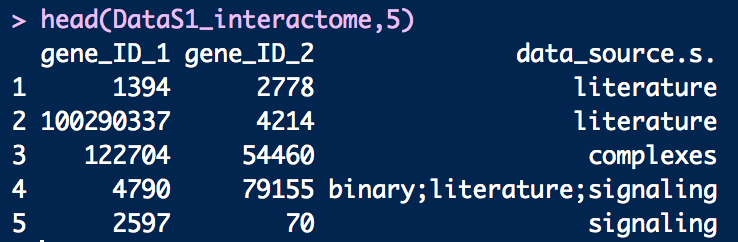
\includegraphics[width=12cm,height=12cm,keepaspectratio]{DataS1.png} containing 141,295 pairs of genes.\\
 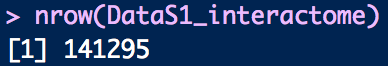
\includegraphics{nrows_interactome.png} \\Here is a summary quantifying the number of instance of each types of interactions and demonstrating how one or more interactions occurs for each gene-gene pair: \\
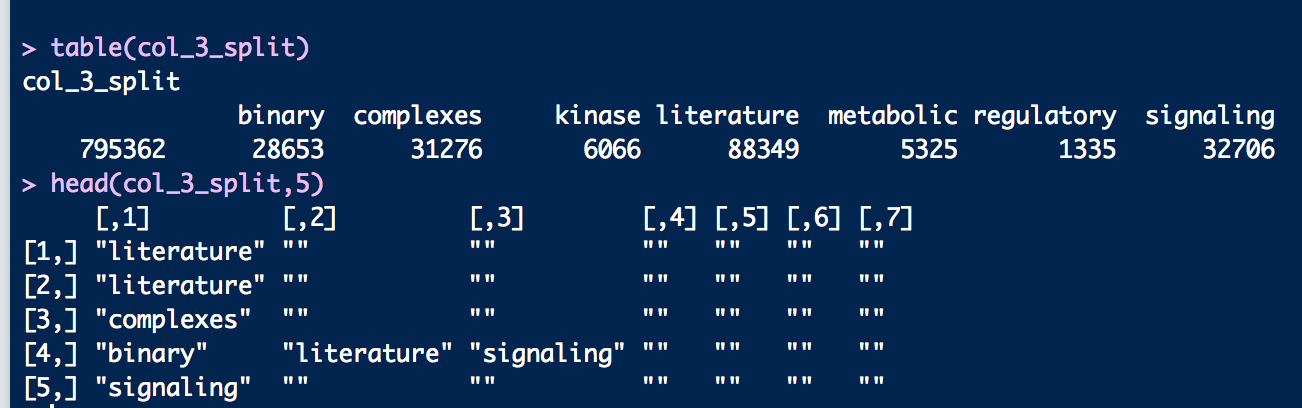
\includegraphics[width=12cm,height=12cm,keepaspectratio]{D1_types_int.png}

\item2) Disease genes dataset.

\item 3) Network properties dataset for the diseases considered in the study. Here are summary statistics describing number of genes ascribed to each disease and other parts of the dataset:\\ 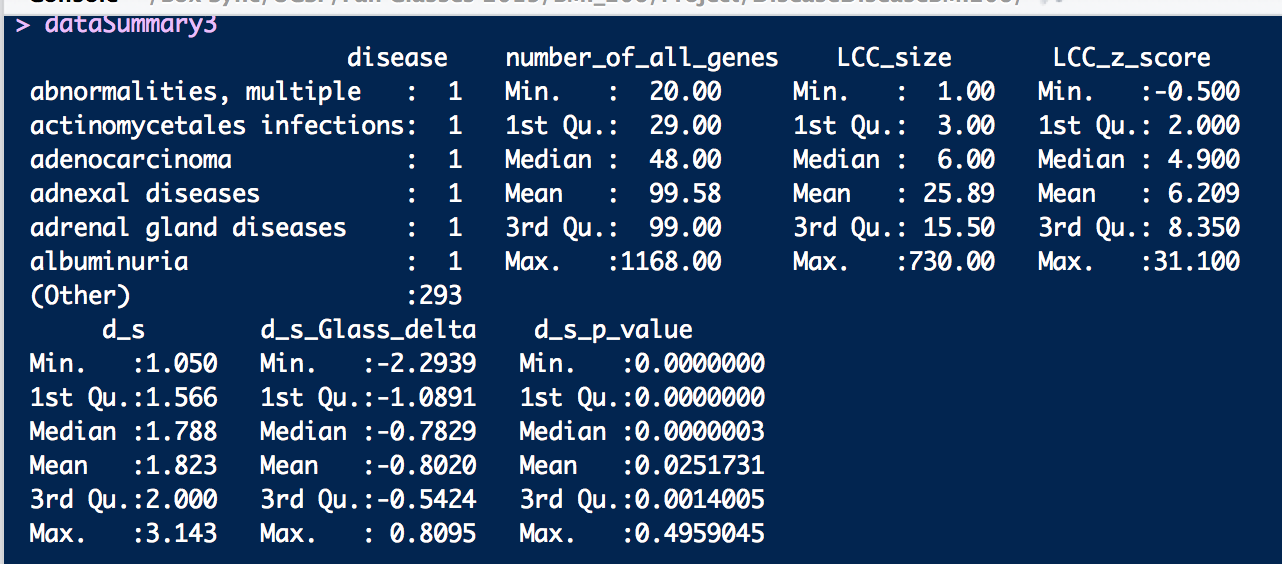
\includegraphics[width=12cm,height=12cm,keepaspectratio]{d3_summ.png}

\item 4) Network relationships for all the pairs of diseases considered in the study, summarized here: \\
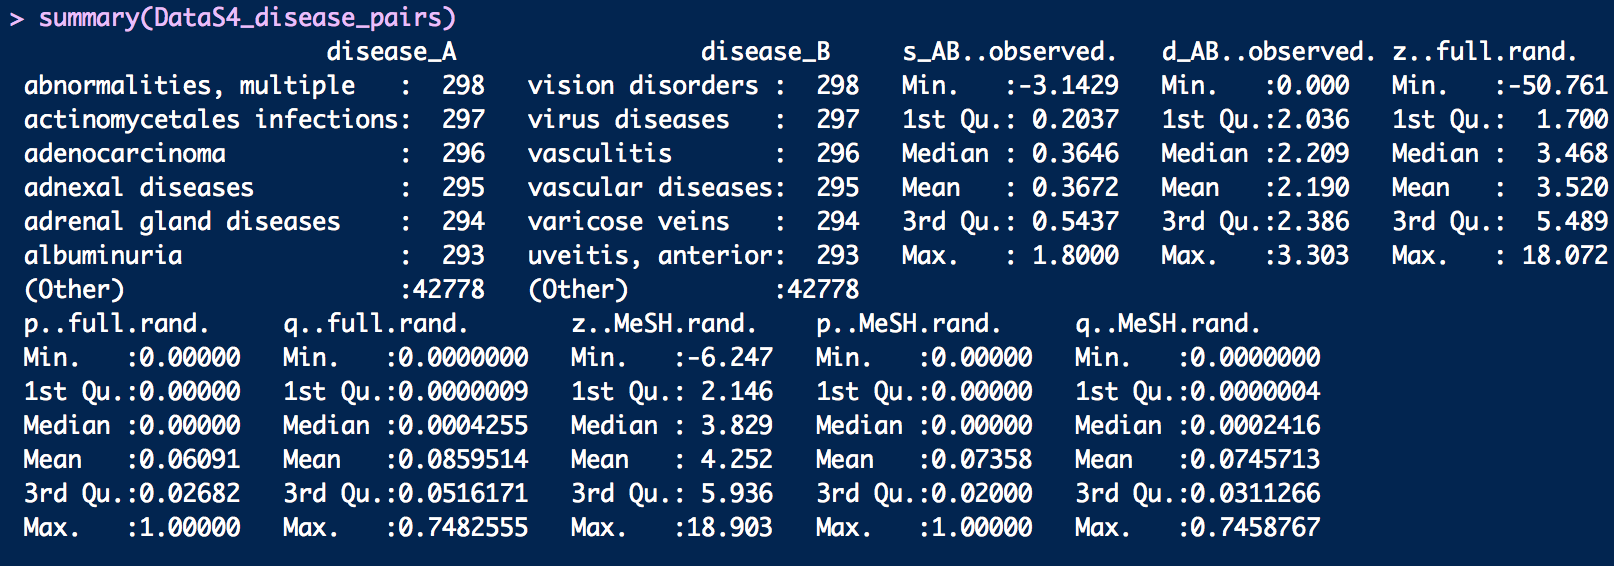
\includegraphics[width=12cm,height=12cm,keepaspectratio]{S4_summ.png}

\end{itemize}

\end{document}  